\documentclass[border=1mm]{standalone}
% \usepackage[margin=2.5cm]{geometry}

\usepackage{graphicx,tikz,tikz-layers,amsmath,ifthen,tabularray,xcolor,fontawesome5} 
\usetikzlibrary{decorations.markings,calc,positioning,arrows,shapes.geometric,arrows.meta,matrix,decorations.text}

\colorlet{myred}{red!80!black}
\colorlet{myblue}{blue!80!black}
\colorlet{mybluee}{myblue!80!black}
\colorlet{mygreen}{green!60!black}
\colorlet{myorange}{orange!70!red!60!black}
\colorlet{mydarkred}{red!20!black}
\colorlet{mydarkblue}{blue!40!black}
\colorlet{mydarkgreen}{green!20!black}




\begin{document}

% \resizebox{\textwidth}{!}{
\tikz[font=\small, scale=1, every node/.style={outer sep=0pt, inner sep=0pt, rounded corners=.5mm, align=center}, w/.style={minimum width=#1}, h/.style={minimum height=#1}, s/.style={minimum size=#1}, eu/.style={shorten >=#1}, ed/.style={shorten <=#1}, line join=round]
{
\tikzset{>={Latex[length=1.5mm, width=1.25mm]}}


\node[draw, w=2cm, h=.9cm, fill=mygreen!15] (pr1) {Perceiver\\Resample};
\node[draw, w=2cm, h=.9cm, fill=mygreen!15, right=.5cm of pr1] (pr2) {Perceiver\\Resample};

\node[w=2cm, h=1.4cm, below=.5cm of pr1] (ve1) {Vision\\Encoder\\\faSnowflake};
\begin{scope}[on behind layer]
\draw[fill=myblue!15] (ve1.south west)--(ve1.south east)--($(ve1.north east)+(-.2,0)$)--($(ve1.north west)+(.2,0)$)--cycle;
\end{scope}

\node[w=2cm, h=1.4cm, below=.5cm of pr2] (ve2) {Vision\\Encoder\\\faSnowflake};
\begin{scope}[on behind layer]
\draw[fill=myblue!15] (ve2.south west)--(ve2.south east)--($(ve2.north east)+(-.2,0)$)--($(ve2.north west)+(.2,0)$)--cycle;
\end{scope}

% Images
\node[below=.5cm of ve1] (dog1) {\includegraphics[width=2cm]{images/mosaic2/Dog5.jpg}};

\node[below=.5cm of ve2] (cat1) {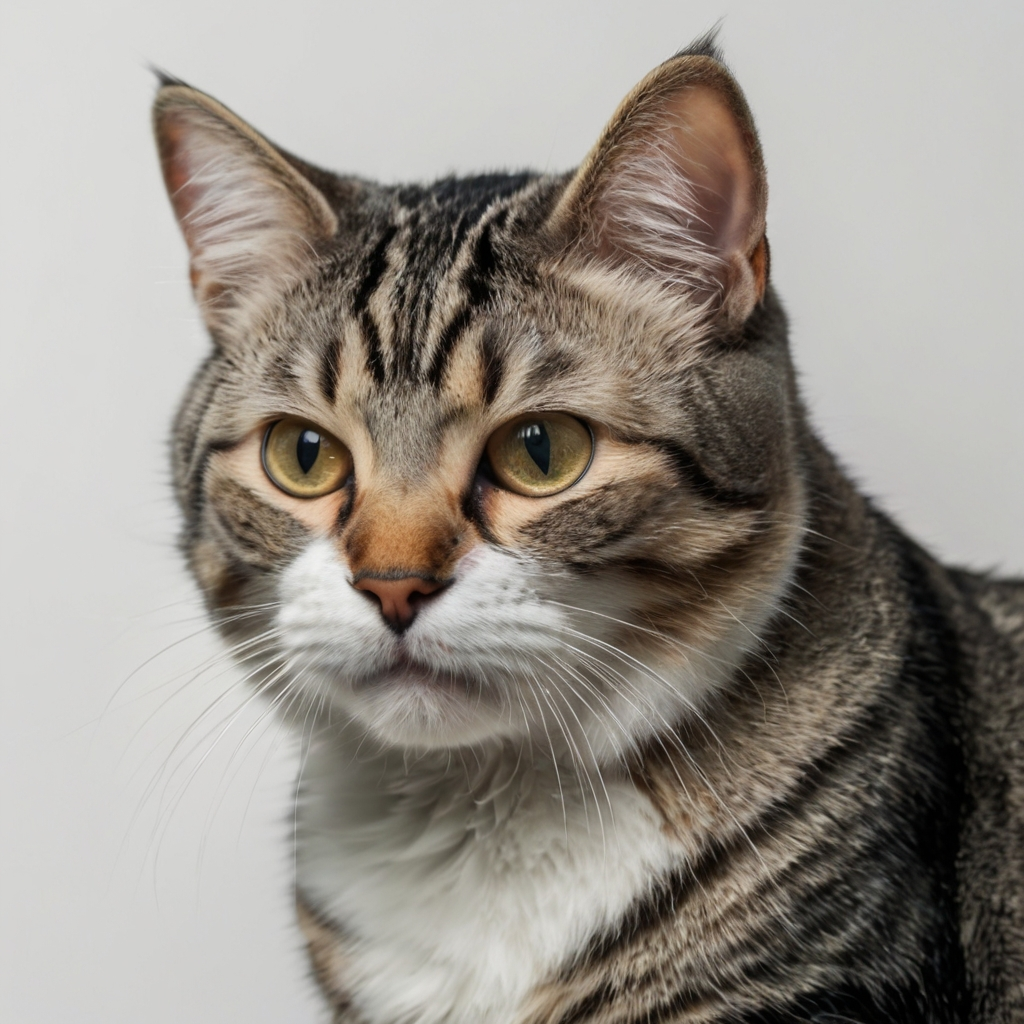
\includegraphics[width=2cm]{images/cat.jpg}};

\node[right=1.5cm of cat1, label={[label distance=1mm]right:This is a very cute dog.}] (dog2) {\includegraphics[width=2cm]{images/mosaic2/Dog5.jpg}};

\node[right=4cm of dog2, label={[label distance=1mm]right:This is}] (cat2) {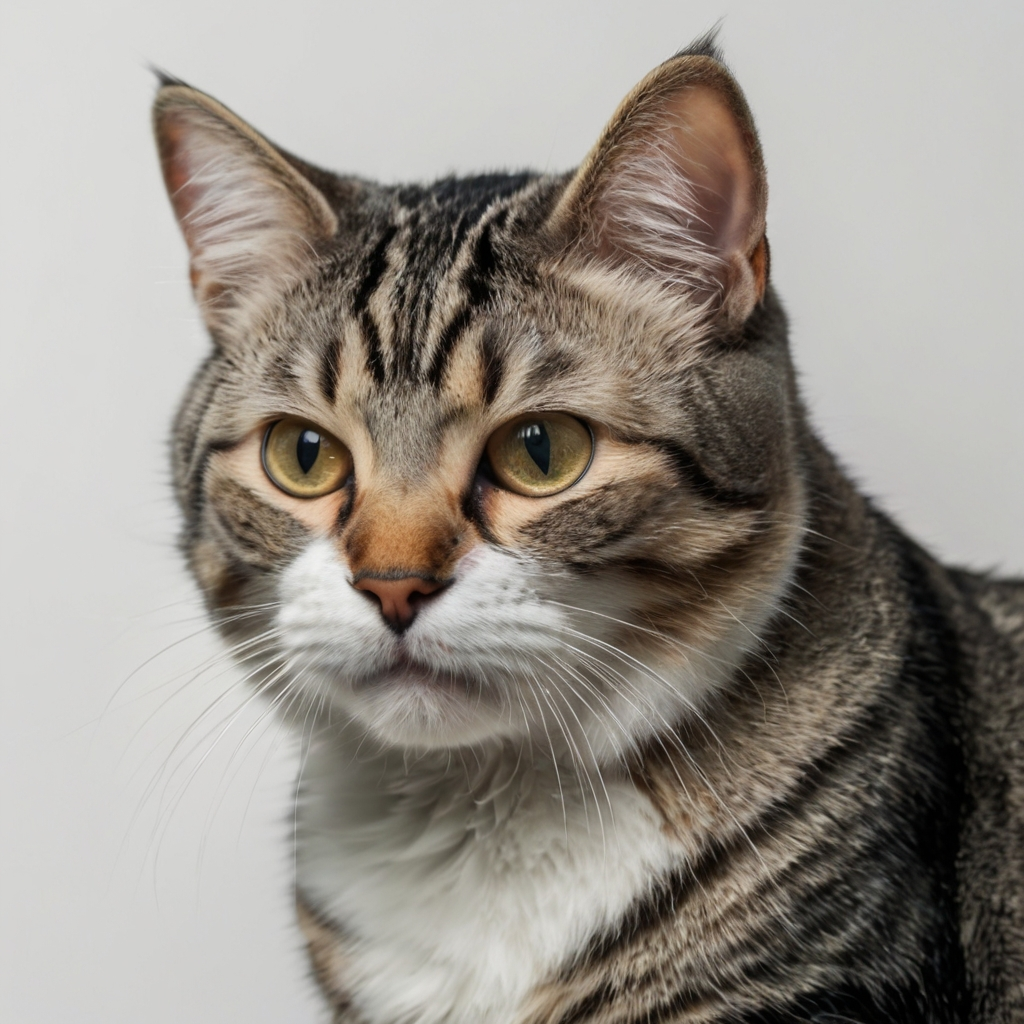
\includegraphics[width=2cm]{images/cat.jpg}};

% Gray background for cat and dog images
\begin{scope}[on behind layer]
\node[fill=gray!20, w=9.5cm, h=2.25cm, anchor=west] (gr) at ($(dog2.west)+(-.2,0)$) {};    
\end{scope}

% Processed text
\node[draw, w=9.5cm, h=.5cm, above=.6cm of gr] (txt) {\texttt{$<$image$>$ This is a very cute dog. $<$image$>$ This is}};

%--
\node[draw, above=.75cm of txt, w=7cm, h=.5cm, fill=mygreen!15] (a) {1st GATED XATTN-DENSE};
\node[draw, above=.2cm of a, w=7cm, h=.5cm, fill=myblue!15] (b) {1st LM block};

\node[draw, above=.5cm of b, w=7cm, h=.5cm, fill=mygreen!15] (c) {n-th GATED XATTN-DENSE};
\node[draw, above=.2cm of c, w=7cm, h=.5cm, fill=myblue!15] (d) {n-th LM block};

% Gray background for GATED blocks
\begin{scope}[on behind layer]
\node[fill=gray!20, w=9.5cm, h=3.25cm] (gr1) at ($(b)!.5!(c)$) {};   
\end{scope}

\node[draw, above=.5cm of d, w=9.5cm, h=.5cm, fill=myred!15] (e) {A very serious cat};

% Legend
\node[draw, w=4.5cm, h=1.75cm, above=1.2cm of {$(pr1.north)!.5!(pr2.north)$}] (box) {};

\node[draw, s=.7cm, anchor=north west, fill=myblue!15, label={[label distance=1mm]right: Pretrained and frozen}] at ($(box.north west)+(.2,-.1)$) {\large\faSnowflake};

\node[draw, s=.7cm, anchor=south west, fill=mygreen!15, label={[label distance=1mm]right: Trained from scratch}] at ($(box.south west)+(.2,.1)$) {};

\node[anchor=east] at ($(b.east)+(-.2,0)$) {\faSnowflake};
\node[anchor=east] at ($(d.east)+(-.2,0)$) {\faSnowflake};

% Arrows
\draw[-] (gr)--(txt);
\draw[->] (txt)--(a);
\draw[] (a)--(b);
\draw[densely dashed] (b)--(c);
\draw[] (c)--(d);
\draw[->] (d)--(e);
\draw[->] (dog1)--(ve1);
\draw[->] (ve1)--(pr1);
\draw[->] (cat1)--(ve2);
\draw[->] (ve2)--(pr2);

% Labels
\node[anchor=south west] at ($(gr.north west)+(0,.1)$) {\textbf{Interleaved visual/text data}};
\node[anchor=south west] at ($(txt.north west)+(0,.1)$) {\textbf{Processed image}};
\node[anchor=south west] at ($(e.north west)+(0,.1)$) {\textbf{Output: text}};

\draw[->] (pr1.north) |- coordinate[pos=.82] (u) ($(c.west)+(0,.12)$);
\draw[->] (pr2.north) |- coordinate[pos=.78] (v) ($(c.west)+(0,-.12)$);

\draw[->] (u) |- ($(b.west)+(0,.12)$);
\draw[->] (v) |- ($(b.west)+(0,.-.12)$);

\draw[->] (cat2.south)--++(0,-.5) -| (cat1);
\draw[->] (dog2.south)--++(0,-.5) -| (dog1);
}

% }



\end{document}
